%% SkyPass -- manuscript for SN Computer Science (Springer Nature).
%%
%% Class line, package list and theorem declarations follow
%% Springer_Nature_LaTeX_Template/sn-article.tex exactly. sn-mathphys-num is the
%% template's own active style and numbers citations in square brackets, which is
%% how this text refers to them.
%%
%% Figures are rendered in Computer Modern to match the sn-jnl body font
%% (experiments/make_figures.py --font cm).

\documentclass[pdflatex,sn-mathphys-num]{sn-jnl}

\usepackage{graphicx}%
\usepackage{multirow}%
\usepackage{amsmath,amssymb,amsfonts}%
\usepackage{amsthm}%
\usepackage{mathrsfs}%
\usepackage[title]{appendix}%
\usepackage{xcolor}%
\usepackage{textcomp}%
\usepackage{manyfoot}%
\usepackage{booktabs}%
\usepackage{algorithm}%
\usepackage{algorithmicx}%
\usepackage{algpseudocode}%
\usepackage{listings}%

%% Added to the template list: the manuscript sets units with siunitx.
\usepackage{siunitx}%
\sisetup{detect-all, per-mode=symbol}%

%% Justified text with a looser tolerance, so long identifiers and URLs do not
%% push words into the margin.
\tolerance=1500
\emergencystretch=2em
\hbadness=4000

\theoremstyle{thmstyleone}%
\newtheorem{theorem}{Theorem}%
\newtheorem{proposition}[theorem]{Proposition}%
\theoremstyle{thmstyletwo}%
\newtheorem{example}{Example}%
\newtheorem{remark}{Remark}%
\theoremstyle{thmstylethree}%
\newtheorem{definition}{Definition}%

\raggedbottom

%%== generated result values (experiments/make_tables.py), inlined ==%%
%% Springer forbids \input, so generated/numbers.tex is pasted here.
% Auto-generated by experiments/make_tables.py -- do not edit.
% Every inline number in the paper resolves through these macros.
\newcommand{\AccOne}{85.1}
\newcommand{\AgeComparisons}{33\,223}
\newcommand{\AgeDayOne}{0.05}
\newcommand{\AgeDayOneMedian}{0.01}
\newcommand{\AgeFortnight}{16.2}
\newcommand{\AgeGrowth}{1.29}
\newcommand{\AgeMonth}{75.3}
\newcommand{\AgeMonthMedian}{13.69}
\newcommand{\AgeObjects}{60}
\newcommand{\AgeWeek}{4.3}
\newcommand{\AgeWeekMedian}{0.70}
\newcommand{\BaseSkew}{1.8}
\newcommand{\BestBudgetMode}{50\% of nights}
\newcommand{\BootResamples}{10\,000}
\newcommand{\BootStations}{6}
\newcommand{\BtwWthRatio}{2.2}
\newcommand{\BudgetBlindClearRate}{13.9}
\newcommand{\BudgetClearRate}{23.1}
\newcommand{\BudgetGainClear}{37.6}
\newcommand{\BudgetGainClearHi}{80.4}
\newcommand{\BudgetGainClearLo}{3.1}
\newcommand{\BudgetGainClearPos}{0.98}
\newcommand{\BudgetGainEV}{19.0}
\newcommand{\BudgetGainEVHi}{24.9}
\newcommand{\BudgetGainEVLo}{9.2}
\newcommand{\BudgetOracleClear}{106.7}
\newcommand{\BudgetOracleEV}{46.0}
\newcommand{\BudgetRecoveredClear}{35}
\newcommand{\BudgetRecoveredEV}{41}
\newcommand{\BudgetTotal}{90}
\newcommand{\CallReduction}{23.7}
\newcommand{\CallsDense}{54\,864\,000}
\newcommand{\CallsFast}{2\,311\,148}
\newcommand{\Capacity}{3}
\newcommand{\ClearThreshold}{30}
\newcommand{\ClearThresholdEval}{30}
\newcommand{\CloudChennai}{88}
\newcommand{\CloudReduction}{0.209}
\newcommand{\DPBigMs}{285.3}
\newcommand{\DPBigN}{100\,000}
\newcommand{\DPOptimalPct}{100.00}
\newcommand{\DemoBright}{367}
\newcommand{\DemoCandidates}{87}
\newcommand{\DemoClear}{85}
\newcommand{\DemoDark}{1297}
\newcommand{\DemoGeometric}{12\,449}
\newcommand{\DemoHorizon}{7}
\newcommand{\DemoObjects}{635}
\newcommand{\DemoRuntime}{109.4}
\newcommand{\DemoScheduled}{26}
\newcommand{\DemoSunlit}{8093}
\newcommand{\DenseAos}{0.504}
\newcommand{\EpochMax}{13.04}
\newcommand{\EpochMean}{0.55}
\newcommand{\EpochMedian}{0.42}
\newcommand{\EpochPninety}{0.95}
\newcommand{\EpochUnderOne}{90.2}
\newcommand{\EvalDays}{60}
\newcommand{\EvalEnd}{2026-08-23}
\newcommand{\EvalObjects}{300}
\newcommand{\EvalStart}{2026-06-25}
\newcommand{\EvalStations}{6}
\newcommand{\EvalStationsWord}{six}
\newcommand{\ForecastDays}{60}
\newcommand{\ForecastEnd}{2026-08-23}
\newcommand{\ForecastStart}{2026-06-25}
\newcommand{\GAGenerations}{120}
\newcommand{\GAPct}{99.67}
\newcommand{\GAPopulation}{60}
\newcommand{\GASites}{6}
\newcommand{\GASlowdown}{38\,922}
\newcommand{\GreedyBestPct}{99.95}
\newcommand{\GreedyElevMin}{9.4}
\newcommand{\GreedyElevOptPct}{62.7}
\newcommand{\GreedyElevPct}{95.39}
\newcommand{\GreedyGain}{\ensuremath{-}60.0}
\newcommand{\GreedyValueMin}{85.9}
\newcommand{\GreedyValuePct}{99.95}
\newcommand{\GreedyWorstPct}{95.07}
\newcommand{\HistBudgetClear}{33.2}
\newcommand{\HistBudgetEV}{19.0}
\newcommand{\HistQuotaClear}{9.2}
\newcommand{\HistQuotaEV}{1.7}
\newcommand{\HistTightClear}{75.9}
\newcommand{\HssOne}{0.347}
\newcommand{\HssPersistence}{0.206}
\newcommand{\HssSeven}{0.114}
\newcommand{\HssThree}{0.289}
\newcommand{\InterceptMax}{0.70}
\newcommand{\InterceptMin}{0.07}
\newcommand{\JaccardDurOnly}{0.86}
\newcommand{\JaccardExtreme}{0.70}
\newcommand{\JaccardMid}{0.89}
\newcommand{\JaccardNinety}{0.70}
\newcommand{\MaeOne}{0.193}
\newcommand{\MaePersistence}{0.212}
\newcommand{\Missed}{4}
\newcommand{\NCatalogue}{635}
\newcommand{\NMatched}{1761}
\newcommand{\NPasses}{1801}
\newcommand{\NSats}{635}
\newcommand{\PassCorr}{0.41}
\newcommand{\ProviderN}{308}
\newcommand{\ProviderObjects}{52}
\newcommand{\ProviderTcaMax}{1.82}
\newcommand{\ProviderTcaMean}{0.041}
\newcommand{\ProviderTcaMedian}{0.00}
\newcommand{\ProviderTcaPninetyfive}{0.176}
\newcommand{\PythonVersion}{3.13.5}
\newcommand{\QuotaGainClear}{\ensuremath{-}0.2}
\newcommand{\QuotaGainClearHi}{3.5}
\newcommand{\QuotaGainClearLo}{\ensuremath{-}11.6}
\newcommand{\QuotaGainClearPos}{0.46}
\newcommand{\QuotaGainEV}{\ensuremath{-}1.5}
\newcommand{\QuotaGainEVHi}{2.0}
\newcommand{\QuotaGainEVLo}{\ensuremath{-}2.7}
\newcommand{\QuotaOracleClear}{31.6}
\newcommand{\QuotaOracleEV}{12.0}
\newcommand{\QuotaRawEV}{\ensuremath{-}9.2}
\newcommand{\RawBudgetClear}{29.9}
\newcommand{\RawBudgetEV}{8.0}
\newcommand{\RawQuotaClear}{\ensuremath{-}5.5}
\newcommand{\Recall}{99.78}
\newcommand{\ScaleDays}{7}
\newcommand{\ScaleObjects}{635}
\newcommand{\ScalePasses}{12\,438}
\newcommand{\ScaleSchedMs}{2.1}
\newcommand{\ScaleSeconds}{104.4}
\newcommand{\SchedTrials}{2000}
\newcommand{\SgpVersion}{2.27}
\newcommand{\SkillStations}{7}
\newcommand{\SkillStationsWord}{seven}
\newcommand{\SkyfieldAos}{0.060}
\newcommand{\SkyfieldTca}{0.055}
\newcommand{\SkyfieldTcaMax}{0.293}
\newcommand{\SlopeChennai}{0.56}
\newcommand{\SlopeMax}{0.61}
\newcommand{\SlopeMin}{0.17}
\newcommand{\StructureDays}{30}
\newcommand{\TightBudget}{45}
\newcommand{\TightClearRate}{28.1}
\newcommand{\TightGainClear}{55.0}
\newcommand{\TightGainClearHi}{144.5}
\newcommand{\TightGainClearLo}{24.7}
\newcommand{\TightGainClearPos}{1.00}
\newcommand{\TightGainEV}{19.2}
\newcommand{\TrainDays}{90}

\begin{document}

\title[Weather-Aware Satellite Pass Scheduling]{SkyPass: Weather-Aware Satellite
Pass Scheduling for Small Ground Stations and the Decision-Dependent Value of
Cloud Forecasts}

\author*[1]{\fnm{Rohith Prem} \sur{S}}\email{rohithprem91@gmail.com}
\author[2]{\fnm{R.} \sur{Selvakumar}}\email{selvakumarr@saveetha.ac.in}

\affil*[1]{\orgdiv{Department of Computer Science and Engineering},
\orgname{Saveetha Engineering College}, \orgaddress{\city{Chennai},
\postcode{602105}, \state{Tamil Nadu}, \country{India}}}

\affil[2]{\orgdiv{Department of Artificial Intelligence and Machine Learning},
\orgname{Saveetha Engineering College}, \orgaddress{\city{Chennai},
\postcode{602105}, \state{Tamil Nadu}, \country{India}}}

\abstract{Observation planning at a small ground station is split across
unconnected tools: one predicts passes, another evaluates optical visibility,
cloud is checked by hand, and overlapping passes are reconciled by the operator.
This work examines whether an integrated, weather-aware planner increases the
number of passes observed under clear sky, and under which operating conditions.
The planner, SkyPass, carries a catalogue of orbital elements through SGP4
propagation, pass extraction by coarse bracketing and bisection, visibility
scoring, cloud-forecast calibration against reanalysis, and exact conflict
resolution, posed as weighted interval scheduling under a nightly budget and
solved exactly by a dynamic program whose running time grows only linearly with the number of candidate passes and with the nightly observation limit. Forecast skill is verified against ERA5
reanalysis at \SkillStationsWord{} stations and scheduling value at
\EvalStationsWord{}, retrospectively over \EvalDays~days. Pass extraction agrees
with an independent implementation to \SkyfieldTca~s while using
\CallReduction$\times$ fewer propagator evaluations than a dense scan, and the
dynamic program matched exhaustive search on all \SchedTrials~randomised
instances. A station required to observe every night gained nothing from the
forecast, whereas one free to select its observing nights raised realised yield
by \BudgetGainEV\% (expected value) and \BudgetGainClear\% (clear-sky count).
Calibration raised the gain in every regime; uncalibrated, the forecast was
worse than ignoring weather under a nightly quota. The value of a forecast
therefore depends on the decision it informs: weather-aware planning pays when a
station may choose its observing nights, and pays most with a calibrated
forecast.}

\keywords{satellite pass prediction, SGP4, ground station scheduling, interval scheduling, forecast calibration, optical observation}

\maketitle

\section{Introduction}

Small ground stations, such as university laboratories, amateur-radio clubs and
individual optical observers, face a recurring planning problem. Several hundred
satellites are potentially observable and generate thousands of passes in a week,
of which only a few dozen merit the operator's time, and the station attends to
one object at a time.

Existing tools address only parts of this. Pass predictors compute rise and set
times from two-line elements (TLEs) and the SGP4
propagator~\cite{vallado2022fundamentals,acciarini2025sgp4}, some adding an
illumination test so that optical observers are not shown daylight passes. A few
display a weather indication beside a pass, but to our knowledge none let the
forecast \emph{rank} passes or drive a scheduling decision, and none resolve
overlapping passes.

Weather is the more consequential omission. At the site used as a running
example (Chennai, India, \ang{12.92}\,N), mean observed cloud over optically
viable passes was \CloudChennai\%, under which most geometrically favourable
passes are not observable, yet a predictor ranking by culmination elevation
recommends an overcast night. The scheduling omission is less apparent:
once several satellites are tracked their passes overlap and a single-aperture
station has to choose. The literature treats that from the operator side of the
link, as spacecraft tasking and range scheduling solved with mathematical
programs, metaheuristics or learning
methods~\cite{li2023srsp,ou2023drl,wang2021agile}, carrying constraints a small
station does not have.

This paper shows that the small-station problem admits a substantially simpler
exact formulation, and that the treatment of weather is what improves realised
outcomes. The contributions are: an integrated pipeline accounting for the
passes removed by each physical constraint; a validated pass extractor; exact
capacity-constrained conflict resolution requiring neither a solver nor a
metaheuristic; a weather claim verified against ERA5
reanalysis~\cite{hersbach2020era5}; and two negative results, namely that
weather-awareness yields no benefit under a fixed nightly quota and that the
uncalibrated forecast degrades performance there.

% ===========================================================================
\section{Related Work}

SGP4 and its two-line element sets remain
the standard basis for rapid position
prediction~\cite{vallado2022fundamentals,acciarini2025sgp4}, with accuracy
limited by the elements rather than the propagator: errors grow with
element-set age, measured against on-board GPS~\cite{kovar2022tle}. Whether a
satellite is \emph{seen} depends on illumination and photometry, treated with a
conical Earth-shadow model~\cite{vallado2022fundamentals} and a diffuse-sphere
phase function~\cite{fankhauser2023brightness}.

Satellite range scheduling is an oversubscribed
combinatorial problem~\cite{li2023srsp}, usually approached with multi-objective
optimisation, metaheuristics or reinforcement learning~\cite{ou2023drl}. Earth
observation scheduling is a large adjacent
literature~\cite{wang2021agile}, in which cloud cover appears as an uncertainty
hedged during imaging tasking~\cite{wang2020robust}, although always on the
\emph{operator} side. Where the structure is single-machine interval selection,
exact polynomial algorithms exist: weighted interval scheduling is a textbook
dynamic program~\cite{cormen2022introduction}.

Professional observatories schedule around
weather with queue schedulers that re-plan as conditions
change~\cite{xie2024astrosa}, but assume an institutional software stack and
on-site sky monitoring. Forecast verification and forecast value are mature
fields~\cite{brown2021met}, and statistical post-processing is essential before a
forecast drives a decision~\cite{vannitsem2021postprocessing}. To our knowledge
that machinery has not been applied to observer-side pass planning.

% ===========================================================================
\section{System Design}
\label{sec:design}

SkyPass is a five-stage pipeline (Fig.~\ref{fig:arch}). Each stage is a pure
function of the preceding one, so any stage may be ablated independently, which
is the mechanism by which the weather claim is evaluated.

\begin{figure}[htbp]
\centering
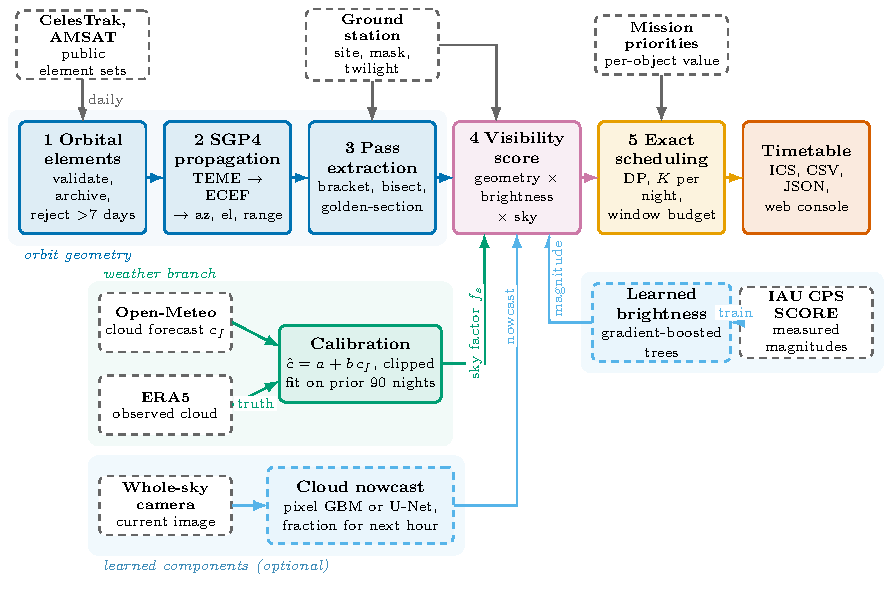
\includegraphics[width=0.72\textwidth]{Fig1}
\caption{SkyPass pipeline. The cloud forecast is calibrated against reanalysis
before it is allowed to influence the score; the scheduler then resolves
conflicts exactly under the station's nightly observing budget.}
\label{fig:arch}
\end{figure}

\subsection{Element sets, propagation and pass extraction}
Element sets are fetched from CelesTrak~\cite{celestrak}, checksum-validated,
deduplicated per NORAD identifier keeping the newest epoch, and \emph{archived
under the date of retrieval}, since CelesTrak serves only current elements and
without a local archive a published prediction cannot be repeated. Sets older
than $\tau_\mathrm{max}$ are rejected. Positions come from the reference SGP4
implementation; the TEME vector is rotated to ECEF by Greenwich mean sidereal
time and converted to topocentric azimuth, elevation and range on the WGS-84
ellipsoid. Polar motion is neglected, being far under the SGP4 error budget, and
refraction is reported but not applied to the horizon mask, so results do not
depend on assumed surface conditions.

Because cost is dominated by propagator calls, pass extraction minimises them.
Elevation is sampled on a coarse grid to \emph{bracket} horizon crossings; since
elevation within a pass is smooth and unimodal, a sign change of
$\varepsilon(t) - \varepsilon_\mathrm{mask}$ between adjacent samples brackets
exactly one crossing. Brackets are refined by bisection to \SI{0.1}{\second} and
culmination by golden-section search. The coarse step is $P/240$ bounded to
\SIrange{5}{30}{\second}, so short-period orbits, whose passes are shortest,
are sampled most finely.

\subsection{Visibility scoring}
Each pass receives a score $S \in [0,1]$ combining a geometric quality term with
multiplicative gates:
\begin{equation}
S = \underbrace{\left(w_e f_e + w_d f_d\right)}_{\text{geometry}}
    \cdot \; f_m \cdot f_s ,
\label{eq:score}
\end{equation}
where $f_e = \min(\varepsilon_\mathrm{max}/\ang{60},1)$ and
$f_d = \min(T/\SI{480}{\second},1)$ saturate culmination elevation and duration,
$f_m$ is a photometric factor and $f_s$ a sky-condition factor.

The multiplicative form is deliberate: an eclipsed pass or one in a bright sky
scores zero irrespective of its geometry, and expected cloud scales the score
down in proportion, which an additive score cannot represent. For optical work the object has to be sunlit and the observer in
darkness; Earth shadow uses the dual-cone
construction~\cite{vallado2022fundamentals}, and apparent magnitude follows the
standard diffuse-sphere relation~\cite{fankhauser2023brightness}
\begin{equation}
m = m_\mathrm{std} + 5\log_{10}\!\frac{d}{\SI{1000}{\kilo\metre}}
    - 2.5\log_{10} F(\psi),
\label{eq:mag}
\end{equation}
with $F(\psi) \propto (\pi-\psi)\cos\psi + \sin\psi$ normalised to $F(0)=1$. In
radio mode the illumination and photometric terms are dropped.

\subsection{Weather integration and calibration}
\label{sec:calib}
The sky factor is $f_s = 1 - \hat{c}$, where $\hat{c}$ is the expected cloud
fraction at culmination, interpolated linearly between hourly samples. Crucially
$\hat{c}$ is \emph{not} the raw forecast, which is heavily over-confident as a
predictor. We fit
\begin{equation}
\hat{c} = \mathbb{E}[c \mid c_f] = a + b\,c_f
\label{eq:calib}
\end{equation}
by least squares on a window that \emph{ends before} the period being planned,
restricted to local night hours, and $\hat{c}$ is clipped to $[0,1]$. The slope
$b$ quantifies the signal: $b \approx
1$ means the forecast can be used directly, $b \approx 0$ that the calibrated
value falls back to site climatology. For the threshold value model the planner instead weights
each pass by the calibrated probability of clear sky,
$P(c \le \theta \mid c_f)$, estimated in ten forecast bins on the same window
and shrunk toward the site's base rate with 20 pseudo-observations, so each value
model is paired with the planner that maximises its expectation.

\subsection{Conflict resolution}
\label{sec:sched}
A single-aperture station observes one object at a time and needs a setup gap
$g$ between targets, so choosing the best mutually compatible subset of passes
is weighted interval scheduling. Writing $v_j = S_j \pi_j$ for the value of pass
$j$ (score times priority), indexing passes $1,\dots,n$ by finish time and
letting $p(j)$ be the largest $i<j$ compatible with $j$ ($0$ if none), the
textbook
recurrence~\cite{cormen2022introduction} gives the exact optimum in $O(n\log n)$.

That alone is insufficient: unconstrained, a station observes every candidate
and weather-awareness has nothing to select. Real stations are limited by
operator and instrument time, so a capacity budget of $K$ observations per night
adds a cardinality dimension:
\begin{equation}
\begin{split}
\mathrm{OPT}[j][k] = \max\bigl(&\mathrm{OPT}[j\!-\!1][k],\\
&v_j + \mathrm{OPT}[p(j)][k\!-\!1]\bigr),
\end{split}
\label{eq:dp}
\end{equation}
with $\mathrm{OPT}[0][k]=\mathrm{OPT}[j][0]=0$. This is exact. The table has one entry for each of the $n$
candidate passes and each count up to the nightly limit $K$, and each entry is
filled in constant time, so after the sort the cost is $O(nK)$: doubling either
the candidates or the limit doubles the work. Observing nights are disjoint,
so applying the budget per night and solving each independently stays exact.
Nights are defined in local solar time, so an evening and the small hours that
follow form one session.

% ===========================================================================
\section{Experimental Setup}
\label{sec:setup}

The catalogue comprises \NCatalogue{} unique objects from CelesTrak GP groups,
checksum-validated and deduplicated, observed from seven stations spanning
distinct cloud climatologies: Chennai and Bengaluru (monsoon), Leh
(high-altitude arid), Tucson (desert), Singapore (equatorial), and Reykjav\'ik
and Svalbard (maritime polar). Unless stated otherwise, the mask is \ang{10}, the
dark-sky threshold \ang{-6} and the setup gap \SI{5}{\minute}. Timing is checked
against a brute-force \SI{1}{\second} dense scan and against
Skyfield~\cite{skyfield}, which shares only the reference SGP4 core with SkyPass. All runs are
single-threaded under Python~\PythonVersion{} with \texttt{sgp4}~\SgpVersion.

All three weather products come from Open-Meteo~\cite{openmeteo}: the
operational forecast, archived past forecasts at lead times of 1--7 days, and
ERA5 reanalysis~\cite{hersbach2020era5} as verification truth. One
methodological point silently invalidates the evaluation if overlooked: the
archive endpoint has to be pinned to the ERA5 model, since at its default it
returns a best-match series which, for recent dates, \emph{is} the archived
forecast, so verifying against it compares a forecast with a copy of itself and
reports a spurious skill of 1.0.

A generative AI assistant (Claude, Anthropic) was used to help edit and
restructure the manuscript text and to write the scripts that build it; the
authors reviewed all such output and take responsibility for the content.

% ===========================================================================
\section{Results}

\subsection{Pass-prediction accuracy and cost}
\label{sec:accuracy}

Table~\ref{tab:accuracy} compares SkyPass against both references over
\NSats{} objects and \NMatched{} matched passes.

\begin{table}[htbp]
\caption{Pass-timing agreement over the full catalogue (635 objects, 1761 matched passes, 24\,h horizon). Values in seconds.}
\label{tab:accuracy}
\centering
\begin{tabular}{lcccc}
\toprule
& \multicolumn{2}{c}{vs.\ 1\,s dense scan} & \multicolumn{2}{c}{vs.\ Skyfield} \\
\cmidrule(lr){2-3}\cmidrule(lr){4-5}
Quantity & mean & p95 & mean & p95 \\
\midrule
$|\Delta t_\mathrm{AOS}|$ & 0.504 & 0.954 & 0.060 & 0.157 \\
$|\Delta t_\mathrm{TCA}|$ & 0.248 & 0.476 & 0.055 & 0.110 \\
$|\Delta t_\mathrm{LOS}|$ & 0.502 & 0.956 & 0.059 & 0.156 \\
$|\Delta \varepsilon_\mathrm{max}|$ (deg) & 0.0008 & 0.0022 & 0.0034 & 0.0102 \\
\bottomrule
\end{tabular}
\end{table}

Against Skyfield, mean agreement is \SkyfieldAos~s on acquisition and
\SkyfieldTca~s on culmination. The apparent \DenseAos~s ``deviation'' from the
dense scan is not SkyPass error: a \SI{1}{\second} grid locates a crossing only
to within its own step, so it lags the true crossing by a mean of
\SI{0.5}{\second}, and the refined estimator is therefore more accurate than the
brute-force reference it is conventionally compared against. The cost difference
is large: \CallsFast{} propagator evaluations against \CallsDense{}, a factor of
\CallReduction. Detection recall is \Recall\%, the residual being very short
grazing transits that peak barely above the mask.

\subsection{Element-set limits on prediction accuracy}
\label{sec:elements}

Sub-second numerical agreement is meaningful only if the elements support that
precision. The median element-set age in the operational catalogue was
\EpochMedian~days (\EpochUnderOne\% under one day). CelesTrak and AMSAT sets
differ by a mean of \ProviderTcaMean~s in culmination over \ProviderN{} matched
passes, but by a median of \ProviderTcaMedian~s: the providers largely
redistribute the same upstream sets, so this is not an independent check. Re-predicting the same passes from progressively
older sets of \AgeObjects{} low-Earth objects gives \AgeComparisons{} aged
comparisons. Within a day of epoch the elements contribute \AgeDayOne~s, the
same order as the \SkyfieldTca~s numerical agreement of
Section~\ref{sec:accuracy}, so neither term dominates; degradation is then
sharply super-linear and heavy-tailed, the mean reaching \AgeWeek~s (median
\AgeWeekMedian~s) at 7--14 days and \AgeMonth~s (median \AgeMonthMedian~s) beyond
a month, so a 5--7 day staleness cutoff suits timing-critical work and daily
element refresh is the largest single lever on prediction accuracy.

\subsection{Skill of the cloud forecast}
\label{sec:forecast}

Weather-aware planning is justified only if the forecast is informative at the
lead times over which an observer plans. Archived forecasts were verified
against ERA5 at all seven stations over \ForecastDays{} days, scoring the
operational decision of whether an hour is clear enough to observe at a
\ClearThreshold\% cloud threshold. Because accuracy misleads when clear hours
are rare, we report the Heidke skill score, a chance-corrected measure in wide
use for categorical verification~\cite{ebert2022rare}. Skill decays from HSS
\HssOne{} at one day to \HssThree{} at three and \HssSeven{} at seven, beating
persistence (\HssPersistence) early but no longer by five to seven days, so a
weather-aware planner is best run on a rolling short horizon. Skill is also
strongly site-dependent, the spread between stations being comparable to the
decay with lead time and lowest at the two monsoon stations: the expected benefit
is a local property rather than a universal constant.

\subsection{Value of weather-aware scheduling}
\label{sec:value}

Five planners select from an identical candidate set, drawn from
\EvalObjects{} objects, at each of \EvalStationsWord{} stations over \EvalDays{}
days (Svalbard has no observable passes), and every timetable is scored against
ERA5. Since the
valuation of a clouded observation is a modelling choice, we report both an
\emph{expected value} model, $\sum_j v_j (1-c_j)$, and a \emph{threshold} model,
$\sum_j v_j \mathbb{1}[c_j \le \theta]$ with $\theta = \ClearThresholdEval\%$.

\begin{figure}[htbp]
\centering
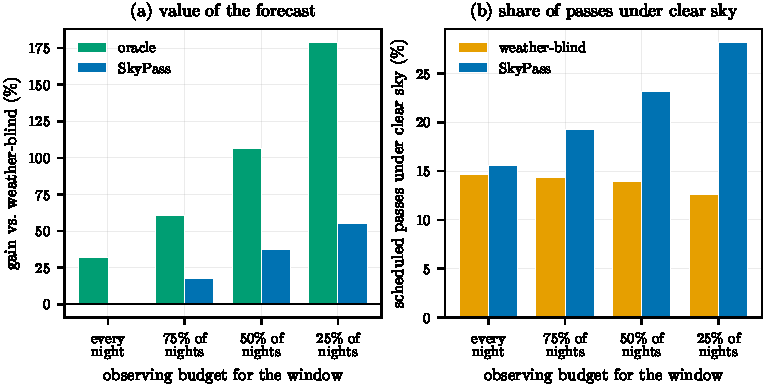
\includegraphics[width=\textwidth]{Fig2}
\caption{Weather-awareness is worth nothing to a station obliged to observe
every night, and a great deal to one that may choose its nights. (a) Gain over
the weather-blind exact planner under the same budget, threshold value model;
the oracle plans with the observed cloud and bounds what any forecast could
achieve. (b) The share of scheduled passes that fell under clear
sky.}
\label{fig:budget}
\end{figure}

Under a fixed nightly quota the forecast yields no benefit: \QuotaGainEV\% and
\QuotaGainClear\% under the two models, against oracle headroom of
\QuotaOracleEV\% and \QuotaOracleClear\%, and the station-bootstrap intervals
of both gains include zero (\QuotaGainEVLo{} to \QuotaGainEVHi\% and
\QuotaGainClearLo{} to \QuotaGainClearHi\%). It is not uninformative, since
forecast and observed cloud correlate at $r = \PassCorr$ at the candidate-pass
timestamps and the clearest-forecast decile does find clearer skies, reducing
observed cloud by $\CloudReduction$. The limitation is that a quota permits only
\emph{reordering within a night}, which two measured properties defeat: cloud is
autocorrelated over the hours a session spans, the between-night standard
deviation being $\BtwWthRatio\times$ the within-night value, while the
ninetieth-percentile pass carries $\BaseSkew\times$ the mean weather-free value.
The score being a product, selecting for clear sky surrenders base value, an
unfavourable exchange when pass quality is the more variable factor.

Given the same cap plus a window budget, so the station may \emph{skip} a night,
the result reverses (Fig.~\ref{fig:budget}): which nights to use is a day-scale
decision, the scale at which the forecast retains skill. We report the central
of the three budget levels as the headline; Fig.~\ref{fig:budget} shows all
four regimes. Observing on \BestBudgetMode{} (\BudgetTotal{} observations),
realised yield improves by
\BudgetGainEV\% and \BudgetGainClear\% (95\% station-bootstrap intervals
\BudgetGainEVLo--\BudgetGainEVHi\% and \BudgetGainClearLo--\BudgetGainClearHi\%),
recovering \BudgetRecoveredEV\% and
\BudgetRecoveredClear\% of the attainable oracle gains; clear-sky passes rise
from \BudgetBlindClearRate\% to \BudgetClearRate\%, and a quarter-of-nights
budget raises the threshold-model gain to \TightGainClear\%
(\TightGainClearLo--\TightGainClearHi\%).

Calibration raises the gain in every regime. Under the quota, supplying
the model cloud field straight to the score costs \QuotaRawEV\% relative to
disregarding weather; under the half budget the raw field still helps
(\RawBudgetEV\% and \RawBudgetClear\%) but less than the calibrated one. Fitted
slopes lie between \SlopeMin{} and \SlopeMax{} and intercepts between
\InterceptMin{} and \InterceptMax{}, so clear forecasts are followed by more
cloud than predicted and cloudy ones by less. Calibration \eqref{eq:calib}
shrinks the forecast toward climatology in proportion to its demonstrated
reliability.

Repeating the evaluation with epoch-correct geometry, that is, with the element
set current on each night, raises the threshold-model gain under the
quota from \QuotaGainClear\% to \HistQuotaClear\% and at a quarter budget from
\TightGainClear\% to \HistTightClear\%, but lowers it at the half budget from
\BudgetGainClear\% to \HistBudgetClear\%, the expected-value gain there being
unchanged at \HistBudgetEV\%. Back-propagated geometry therefore does not
inflate the result systematically, although it is not uniformly conservative.

\subsection{Conflict resolution in practice}
\label{sec:schedresults}

On \SchedTrials{} randomised instances small enough to enumerate exhaustively,
the dynamic program matched the optimum in \DPOptimalPct\% of cases. Greedy
selection \emph{by the score itself} attains \GreedyValuePct\% on average, so
the dynamic program buys little in the average case; its advantage is being
exact at negligible cost with no adverse case. The rules an operator applies
fare worse, optimising a proxy rather than the objective: selection by highest
culmination attains \GreedyElevPct\% on average, is optimal in only
\GreedyElevOptPct\% of instances and falls to \GreedyElevMin\% at worst. An
order-based genetic algorithm of the type common in the satellite-tasking
literature (population \GAPopulation, \GAGenerations{} generations) reaches
\GAPct\% of the optimum but needs roughly \GASlowdown$\times$ more time, a ratio
that depends on that search budget; once the observer-side
problem is recognised as interval scheduling, an exact polynomial solution is
available and a metaheuristic is unnecessary. Scheduling is not the bottleneck in
any case, the dynamic program handling \DPBigN{} candidates in \DPBigMs~ms
against the seconds to minutes propagation needs.

\subsection{End-to-end behaviour}
\label{sec:pipeline}

The funnel is steep and physically interpretable (Fig.~\ref{fig:funnel}): at the
demonstration site \DemoGeometric{} geometric passes reduce to \DemoSunlit{}
sunlit, \DemoDark{} in darkness, \DemoBright{} bright enough to detect,
\DemoCandidates{} above the score floor once forecast cloud is weighted in, and
\DemoScheduled{} scheduled, where a weather-blind tool would present the earlier,
far larger counts. Per-station
runs also check the physics: Svalbard (\ang{78.2}\,N) returns the most geometric
and sunlit passes of any station yet \emph{zero} observable ones, the Sun never
falling below the \ang{-6} threshold in the planned week (29 August to
5 September).

\begin{figure}[htbp]
\centering
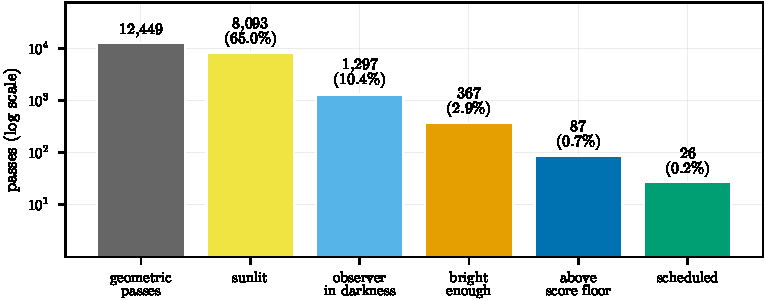
\includegraphics[width=\textwidth]{Fig3}
\caption{Visibility funnel for the demonstration station: of \DemoGeometric{}
geometric passes over \DemoHorizon{} days, \DemoScheduled{} survive to the
timetable. Cloud enters the score as a continuous weight rather than a hard
cut, so the penultimate stage is the score floor.}
\label{fig:funnel}
\end{figure}

Planning \DemoObjects{} objects over \DemoHorizon{} days takes \DemoRuntime~s
single-threaded, dominated by propagation, which scales linearly in objects and
horizon. The timetable is stable against the score weights: varying $w_e$ from
0.3 to 0.7 leaves a Jaccard overlap of at least \JaccardMid{} with the default,
falling to \JaccardNinety{} once elevation dominates ($w_e \ge 0.9$) and to
\JaccardDurOnly{} with duration alone; within the moderate range the physical
constraints, not the weighting, govern the outcome.

% ===========================================================================
\section{Discussion and Limitations}
\label{sec:discussion}

Cloud cover is an imperfect proxy for observing conditions: total cloud
fraction on a reanalysis grid cell of order \SI{25}{\kilo\metre} describes one
line of sight only coarsely, and transparency, seeing, cloud height and aerosol are not modelled. A local
all-sky camera could supply a better nowcast, to which the calibration of
Section~\ref{sec:calib} would apply unchanged, and sub-hourly skill is the route
to the one regime in which the present forecast gives no benefit.

The weather-value gains are pooled over \EvalStationsWord{} stations and
\EvalDays{} nights in one season. A cluster bootstrap that resamples whole
stations (\BootResamples{} draws) gives the 95\% intervals quoted in
Section~\ref{sec:value}; with only \EvalStationsWord{} clusters these intervals
are approximate and probably too narrow, and the difference between the
calibrated and raw planners, whose intervals overlap, was not tested separately.

Both value models are reported because they disagree, and neither
captures partial credit; a station with a specific instrument is better served by
its own value function, which the scheduler accepts unchanged. One instrument
observing one object at a time is assumed, so multiple apertures or a station
network would need a different algorithm. Photometry is approximate,
\eqref{eq:mag} treating every object as a diffuse sphere, so the magnitude gate
is an ordering rather than a prediction, and the ageing measurement is
single-season and limited to low Earth orbit.

% ===========================================================================
\section{Conclusion}

SkyPass integrates pass prediction, optical visibility analysis, cloud-forecast
reasoning and exact conflict resolution into one planner deployable at a small
ground station, producing a timetable that exports to a calendar or a rotator
controller. Pass extraction agrees with an independent implementation to
\SkyfieldTca~s while requiring \CallReduction$\times$ fewer propagator calls
than dense sampling, and conflict resolution is exact at negligible cost.

Two weather findings bear on the design of such systems. First, a forecast is
informative about which \emph{nights} merit observation and much less so for
ranking passes within a night, where cloud is autocorrelated and pass quality
varies more than sky conditions: a planner under a fixed nightly quota gains
nothing, whereas given a budget to allocate selectively the same forecast yields
\BudgetGainEV\% (expected value) and \BudgetGainClear\% (clear-sky count).
Second, calibration against reanalysis raises the gain in every regime tested,
and under a quota it is the difference between a loss and break-even. Both
findings should carry over to other small facilities allocating scarce effort
under uncertain sky, though only one setting is tested here: forecast value is a
property of the decision it informs rather than of the forecast alone.

\backmatter

\section*{Acknowledgements}
The authors thank the Department of Artificial Intelligence and Machine Learning
and the Department of Computer Science and Engineering, Saveetha Engineering
College, Chennai, for their support of this work, which uses public orbital
element sets from CelesTrak and AMSAT and weather data from Open-Meteo.

\section*{Statements and Declarations}

\subsection*{Funding}
No funding was received for conducting this study.

\subsection*{Competing interests}
The authors have no competing interests to declare that are relevant to the
content of this article.

\subsection*{Ethics approval and consent}
Not applicable: the study involves no human participants, human data or animals.

\subsection*{Data and code availability}
SkyPass is open source under the MIT licence at
\url{https://github.com/rohithprem18/skypass}, with the element sets used and
the raw experiment outputs behind every reported value. Weather series are
retrieved from Open-Meteo's public archive by the released scripts; historical
element sets for the ageing and epoch-correct experiments come from Space-Track,
which requires a free account, and are not redistributed.

\bibliography{references}

\end{document}
